\documentclass[article]{jss}

%%%%%%%%%%%%%%%%%%%%%%%%%%%%%%%
%%% declarations for jss.cls %%
%%%%%%%%%%%%%%%%%%%%%%%%%%%%%%%

\author{Matthew K. Lau\\Harvard Forest\\Harvard University\\ \And
        Stuart R. Borrett\\Department of Biology and Marine Biology\\
        University of North Carolina Wilmington\\and\\Duke Network
        Analysis Center\\Social Science Research Institute\\Duke University}
\title{enaR: Ecosystem Network Analysis with R}

%% for pretty printing and a nice hypersummary also set:
\Plainauthor{Matthew K. Lau, Stuart R. Borrett} %% comma-separated
\Plaintitle{enaR: Ecosystem Network Analyses with R} %% without formatting
\Shorttitle{\pkg{enaR}: Ecosystem Network Analyses with R} %% a short title (if necessary)

%% an abstract and keywords
\Abstract{
  Ecosystem Network Analysis (ENA) provides a framework for
  investigating the structure, function and dynamics of ecological
  systems, primarily ecosystem models with physically conserved
  units. We present the \textit{enaR} package, which provides a
  broad representation of many of the core tools developed by the ENA
  community, detailing how to use the primary functions of the package
  for the analysis of single models or simultaneous, synthetic
  analysis of multiple ecosystem models.
}
\Keywords{ecology, ENA, ecosystems, species interactions, networks, \proglang{R}}
\Plainkeywords{ecology, ENA, ecosystems, species interactions, networks, R} %% without formatting
%% at least one keyword must be supplied

%% publication information
%% NOTE: Typically, this can be left commented and will be filled out by the technical editor
%% \Volume{50}
%% \Issue{9}
%% \Month{June}
%% \Year{2012}
%% \Submitdate{2012-06-04}
%% \Acceptdate{2012-06-04}

%% The address of (at least) one author should be given
%% in the following format:

\Address{
  Matthew K. Lau\\
  Harvard Forest\\
  Harvard University\\
  324 N Main St, Petersham, MA 01366, USA\\
  E-mail: \email{matthewklau@fas.harvard.edu}\\
  URL: \url{https://github.com/MKLau}\\
  \\
  Stuart R. Borrett\\
  Department of Biology and Marine Biology\\
  University of North Carolina Wilmington\\
  601 South College Road, Wilmington, NC 28403, USA\\
  E-mail: \email{borretts@uncw.edu}\\
  URL: \url{http://people.uncw.edu/borretts/}
}

%% It is also possible to add a telephone and fax number
%% before the e-mail in the following format:
%% Telephone: +43/512/507-7103
%% Fax: +43/512/507-2851

%% for those who use Sweave please include the following line (with % symbols):
%% need no \usepackage{Sweave.sty}

\usepackage[super, sort]{natbib}
  \bibpunct{(}{)}{;}{a}{,}{,} % required for natbib
\usepackage{ucs} %needed for R output: signif stars etc, quotes
\usepackage[utf8x]{inputenc}
\usepackage[T1]{fontenc}
\usepackage{sidecap}
\usepackage{color}

\newcommand{\R}{\textbf{R}}

%% end of declarations %%%%%%%%%%%%%%%%%%%%%%%%%%%%%%%%%%%%%%%%%%%%%%%


\begin{document}
\Sconcordance{concordance:enaR-vignette.tex:/N/u/mklau/Mason/projects/enaR_development/docs/jss/enaR-vignette.Rnw:%
1 193 1 1 6 1 4 31 1 1 2 4 0 1 2 2 1 1 2 1 0 1 1 3 0 1 2 2 1 1 %
2 4 0 1 2 4 1 1 9 104 1 1 4 3 0 1 2 1 0 1 2 1 0 1 2 1 0 1 5 9 0 %
1 2 23 0 1 2 4 1 1 2 6 0 1 1 5 0 1 1 6 0 1 2 5 1 1 2 11 0 1 2 5 %
1 1 2 30 0 1 2 38 1 1 3 2 0 1 1 1 2 8 0 1 1 7 0 1 2 1 0 1 1 1 2 %
84 0 1 2 166 1 1 3 2 0 1 1 1 2 1 0 1 2 4 0 1 2 4 1 1 3 2 0 1 2 %
1 0 1 2 1 0 1 1 1 2 1 0 1 17 16 0 1 2 4 0 1 2 2 1 1 -39 1 35 1 %
11 19 1 1 2 1 0 1 1 3 0 1 2 5 1 1 2 39 0 1 2 2 1 1 2 1 0 1 1 3 %
0 1 2 10 1 1 2 4 0 1 2 29 1 1 2 1 0 1 3 13 0 1 3 12 0 1 5 19 1 %
1 2 4 0 1 2 61 1 1 3 7 0 1 3 6 0 1 3 4 0 1 2 46 1 1 2 1 0 1 1 6 %
0 1 1 9 0 1 2 74 1 1 2 1 0 1 1 6 0 1 1 10 0 1 2 1 0 1 1 1 2 13 %
0 1 2 4 1 1 2 1 0 1 1 11 0 1 1 3 0 1 2 4 1 1 2 13 0 1 2 34 1 1 %
2 10 0 1 2 34 1 1 2 1 0 1 1 6 0 1 1 11 0 1 2 69 1 1 2 1 0 2 1 7 %
0 1 2 45 1 1 2 1 0 1 1 6 0 1 1 22 0 1 2 5 1 1 2 1 0 1 1 16 0 1 %
2 4 1 1 2 1 0 1 1 19 0 1 2 14 1 1 2 1 0 1 1 6 0 1 1 9 0 1 2 33 %
1 1 2 1 0 1 1 6 0 1 1 6 0 1 2 6 1 1 2 1 0 1 1 6 0 1 1 19 0 1 2 %
48 1 1 2 1 0 1 1 8 0 1 2 6 0 1 2 7 0 1 2 50 1 1 4 1 2 1 0 1 1 8 %
0 1 2 19 0 1 2 44 1 1 2 1 0 1 2 72 0 1 2 3 1 1 2 1 0 1 1 7 0 1 %
2 13 1 1 2 1 0 1 2 1 1 21 0 1 2 13 0 1 2 6 1 1 3 2 0 1 2 1 0 1 %
5 4 0 1 4 3 0 1 2 4 0 1 2 2 1 1 -4 1 8 22 1 1 3 7 0 1 2 1 0 1 2 %
1 0 1 2 6 0 1 2 1 0 1 2 6 0 1 1 5 0 1 2 4 0 1 2 19 1 1 2 4 0 1 %
2 7 1 1 3 16 0 1 3 15 0 1 6 4 0 1 2 6 0 1 3 1 0 1 4 88 0 1 2 3 %
1 1 6 1 3 2 0 1 2 12 0 1 2 1 1 1 4 6 0 1 2 4 1 1 3 2 0 1 1 1 2 %
22 0 1 1 5 0 1 1 11 0 1 2 5 1 1 2 1 0 1 2 1 0 1 1 1 2 1 0 1 4 3 %
0 2 1 1 5 4 0 1 2 4 0 1 2 3 1 1 -5 1 9 41 1 1 2 6 0 1 2 6 0 1 2 %
6 1 1 2 1 0 1 2 1 0 1 2 1 0 1 1 22 0 1 2 1 0 1 2 1 1 1 5 4 0 1 %
2 4 0 1 2 2 1 1 -16 20 0 1 12 1 0 1 8 7 1 1 2 6 0 1 2 5 0 1 2 6 %
0 1 2 8 1 1 2 1 0 1 2 1 0 1 3 1 0 1 1 3 0 1 2 5 1 1 -7 1 11 2 1 %
1 3 8 0 1 3 12 0 1 3 6 0 1 3 6 0 1 3 6 0 1 1 5 0 1 1 5 0 1 1 5 %
0 1 1 5 0 1 2 5 0 1 3 4 0 1 2 11 1 1 2 1 0 1 1 3 0 1 2 26 1}



%%%%Re-organization based on SRB notes

%%%%
%%Intro
%%Ecosystem Networks purpose and structure of models
%%1.network ecology
%%2.ENA
%%3.previous software and enaR

\section[Introduction]{Introduction}
% p1:  intro paragraph (5/7/2015)
Network models have provided an in-road to a variety of complex systems \cite{watts1998collective, newman01scientific01, barabasi12, newman06structure, wasserman1994}, and
although the network approach has deep roots (get old cite from
Mutualistic Networks Book), its use has been expanding rapidly in a
variety of disciplines including ecology \citep{borrett14_rise, ings2009}.  This is due in
part to the flexibility of the core representation, its utility in
answering relational questions, and its applicability to ``Big Data''
problems.  Some scientists are working to build a science of networks \citep{nrc06network, brandes13}.

% p2: Ecosystem Network Analysis
% what, why, bit of history -- two schools

Ecosystem ecologists have developed and used network modeling and analysis for several decades \citep{borrett12_netecol,ulanowicz86,fath99_review}.  From this work, a family of algorithms used to investigate the structure and function of ecological systems has been termed Ecosystem Network Analysis (ENA).  For this approach the network models are comprised of
transfers of thermodynamically conserved energy or matter (represented by weighted, directed graph edges)
between nodes that represent species, groups of species, or non-living components (e.g.,
dead organic matter) of the ecosystem.  The analysis
has been used in a variety of ways, including to show the relative
importance of indirect effects in ecosystems \citep{patten83,
  higashi89, salas11_did} and their capacity to effectively transform
the relations among organisms \citep{ulanowicz90, patten91, fath98,
  bondavalli99}.  From these applications a new theoretical
understanding of ecosystems has emerged \citep{higashi91, belgrano05,
  jorgensen07_newecology}.  Recently, scientists have been applying
these methods to understand trophic dynamics in the Sylt-R{\o}m{\o}
Bight \citep{baird04_sylt,baird08_sylt}, biogeochemical cycling in
estuaries \citep{christian03, hines12}, and urban sustainability
\citep{zhang10, chen12}.

% Orientation
The ENA methodology is an application and extension of economic
Input--Output Analysis \citep{leontief1936,leontief66} that was first
introduced into ecology by \citet{hannon73}.  Since this introduction, two major schools have
developed in ENA \citep{scharler09comparing}.  The first is based on Dr.\ Robert E.\ Ulanowicz's
work with a strong focus on trophic dynamics and a use of information
theory \citep{ulanowicz86, ulanowicz97, ulanowicz04}.  The second
school has an environment focus and is built on the environ concept
introduced by Dr.\ Bernard C.\ Patten \citep{patten76, patten78,
  fath99_review}.  Patten's approach has been collectively referred to
separately as \emph{Network Environ Analysis}. At the core the two
approaches are very similar; however, they make some different
starting assumptions and follow independent yet braided development
tracks. One example difference that has historically inhibited
collaboration and applications is that the two schools orient their
analytical matrices in different ways.  The Ulanowicz school orients
their matrices as flows from rows-to-columns, which is the most common
orientation in the broader field of network science
\citep[e.g.,][]{brandes05}.  In contrast, the Patten School has
historically oriented their matricies from column-to-row.  Recent
research has started to bring the work of the two schools back
together \citep[e.g.,][]{scharler09comparing}; we hope this software
contributes to this.


% p3: Extant Software & The Current Problem
Disparate software packages have been created to support
ENA. Initially algorithms were developed and distributed as the DOS
based NETWRK4 \cite{ulanowicz91}, which is still available from
\url{http://www.cbl.umces.edu/~ulan/ntwk/network.html}.  Some of these
algorithms were re-implemented in an Microsoft Excel based toolbox,
WAND \cite{allesina04_wand}. The popular Ecopath with Ecosim software
that assists with model construction \citep{christensen04} also
provides multiple ENA algorithms. \citet{fath06} published NEA.m that
collects many ENA algorithms together in a single MATLAB\copyright
function. Similarly, the online package by EcoNet (Kazanci 2007) has
also made many of the core ENA algorithms available in an easy access
framework.  Although these packages collectively provide access to a
large set of powerful analytical tools, the fragmented distribution of
these algorithms has inhibited the development of theory and the
further implementation of important algorithms.

{\color{red} MKL: Stuart, I'm not sure what Latham's software is?}


% p4: Objectives (Software & Paper).
The \textit{enaR} package brings together ENA algorithms into one
common software framework that is readily available and extensible.
The package is written in the \R\ language, which is free and
open-source.  Due largely to this, \R\ is now one of the most widely
used analytical programming languages in the biological
sciences. \textit{enaR} builds on existing \R\ packages for
network analysis. For example, it uses the \textit{network} data
structure developed by \citet{butts08_network} and the network
analysis tools built into the \textit{network}, \textit{sna} (social
network analysis) \citep{butts08_social}, and other packages
collectively called \textit{statnet} \citep{handcock2008statnet}. In
this article we introduce the user to ENA concepts and algorithms,
provide description of how to input ecosystem network models and give
detailed description of how to conduct these analyses using
\textit{enaR}.






%%% \subsection{enaR workflow}
% 1. Get a model
% 2. Input/Import model 
% 3. Balance
% 4. Plot
% 5. Analyze structure = static properties
% 6. Analyze flow = dynamic properties
% 7. Other more detailed analyses of structure and dynamics
%    i. control, ii. utility, iii. ascendency, vi. trophic impacts,
%    v. environ, vi. input vs output perspectives
% 8. orientation
% 9. Model library and batch processing
% 10. Connections to other packages
%    i. sna,. ii. igraph, iii. econet
%    any package that uses network representations


%%ENA network models
%%1. describe models
%%2. model construction
%%3. mathematical description

\section{Model Data}

ENA is applied to a network model of energy--matter exchanges among
system components.  The system is modeled as a set of $n$ compartments
or nodes that represent species, species-complexes (i.e., trophic
guilds or functional groups), or non-living components of the system
in which energy--matter is stored.  Nodes are connected by $L$
observed fluxes, termed directed edges or links.  This analysis
requires an estimate of the energy--matter flowing from node $i$ to
$j$ over a given period, $\mathbf{F}_{n\times n}=[f_{ij}]$,
$i,j=1,2,\ldots,n$.  These fluxes can be generated by any process such
as feeding (like a food web), excretion, and death.  As ecosystems are
thermodynamically open, there must also be energy--matter inputs into
the system $\mathbf{z}_{1 \times n}=[z_i]$, and output losses from the
system $\mathbf{y}_{1 \times n}=[y_i]$.  While the Patten School treats
all outputs the same, the Ulanowicz School typically partitions
outputs into respiration $\mathbf{r}_{1\times n}=[r_i]$ and export
$\mathbf{e}_{1\times n}=[e_i]$ to account for differences in energetic
quality. Note that $y_i = r_i + e_i, \forall i$.  Some analyses
also require the amount of energy--matter stored in each node (e.g.,
biomass), $\mathbf{X}_{1\times n}=[x_i]$.  The final required
information is a categorization of each node as living or not, which
is essential for algorithms from the Ulanowicz School.  For
our implementation, we have created a logical vector $\mathbf{Living}_{1 \times
  n}$ that indicates whether the $i^{th}$ node is living (TRUE)
or not (FALSE).  Together, the model data $\mathcal{M}$ can be
summarized as $\mathcal{M} =
\{\mathbf{F}, \mathbf{z}, \mathbf{e}, \mathbf{r}, \mathbf{X}, \mathbf{Living}\}$.



Notice the row-to-column orientation of $\mathbf{F}$.  This is
consistent with the Ulanowicz School of network analysis, as well as
the orientation commonly used in Social Network Analysis and used in
the \textit{statnet} packages.  However, this is the opposite
orientation typically used in the Patten School of analysis that
conceptually builds from a system of differential equations and thus
uses the column-to-row orientation common in this area of
mathematics. Even though the difference is only a matrix transpose,
this single difference may be the source of much confusion in the
literature and frustration on the part of users.  We have selected to
use row-to-column orientation for our primary data structure, as it is
the dominant form across network analytics as evidenced by it use in
the \textit{statnet} packages. The package algorithms also return the
results in the row-to-column orientation by default; however, we have
built in functionality with \texttt{get.orient} and
\texttt{set.orient} that allows users to return output in the Patten
School row-to-column orientation (see Section~\ref{sec:orient} for
details).

\section{Getting Started}

In this section we describe the data necessary for the Ecological
Network Analysis and show how to build the central network data object
in \R\ that contains the model data for subsequent analysis.  To
start, the current stable version can be installed from CRAN:

\begin{Schunk}
\begin{Sinput}
> install.packages('enaR')
\end{Sinput}
\end{Schunk}

The beta version can be installed from GitHub:

\begin{Schunk}
\begin{Sinput}
> library(devtools)
> install_github('SEELab/enaR',ref='beta')
\end{Sinput}
\end{Schunk}

You can now load the package:

\begin{Schunk}
\begin{Sinput}
> library(enaR)
\end{Sinput}
\end{Schunk}

%%%%% Getting Set Up %%%%%%%%%%%
\setkeys{Gin}{width=0.55\linewidth}





% Network Data Object
\subsection{Network Data Class}

The \textit{enaR} package stores the model data in the \textbf{network}
class defined in the \textit{network} package \citep[see][for
details]{butts08_network}. Again, the primary network object
components are:

\begin{itemize}
\item F = flow matrix oriented row-to-column
\item z = inputs
\item r = respiration
\item e = exports
\item y = respiration+exports
\item X = biomass or storage values
\item Living = logical vector indicating if the node is living
  (TRUE) or non-living (FALSE)
\end{itemize}

\subsection{Building a Network Object}

Users can assemble the necessary data elements and then use the
\texttt{pack} function to create the network data object.  Here is an
example of doing this with hypothetical data.

%% PACK A MODEL
\begin{Schunk}
\begin{Sinput}
> ## Generate the flow matrix
> flow.mat <- array(abs(rnorm(100,4,2))*sample(c(0,1),100,replace=TRUE),
+                    dim=c(4,4))
> ## Name the nodes
> rownames(flow.mat) <- colnames(flow.mat) <- paste('node',(1:nrow(flow.mat)),sep='')
> ## Generate the inputs
> inputs <- runif(nrow(flow.mat),0,4)
> ## Generate the exports
> exports <- inputs
> ## "Pack" the model into a network object
> fake.model <- pack(flow=flow.mat,
+                     input=inputs,
+                     export=exports,
+                     living=TRUE)
\end{Sinput}
\begin{Soutput}
[1] "respiration" "storage"    
\end{Soutput}
\begin{Sinput}
> ## The model network object contents
> fake.model
\end{Sinput}
\begin{Soutput}
 Network attributes:
  vertices = 4 
  directed = TRUE 
  hyper = FALSE 
  loops = TRUE 
  multiple = FALSE 
  bipartite = FALSE 
  balanced = FALSE 
  total edges= 6 
    missing edges= 0 
    non-missing edges= 6 

 Vertex attribute names: 
    export input living output respiration storage vertex.names 

 Edge attribute names: 
    flow 
\end{Soutput}
\end{Schunk}

The individual components can be extracted from the data object using
the form specified in the \textit{network} package.  For example, we
can pull out node of vertex attributes as follows:

\begin{Schunk}
\begin{Sinput}
> fake.model%v%'output'
\end{Sinput}
\begin{Soutput}
[1] NA NA NA NA
\end{Soutput}
\begin{Sinput}
> fake.model%v%'input'
\end{Sinput}
\begin{Soutput}
[1] 0.7630464 3.5304482 2.7436423 3.2868305
\end{Soutput}
\begin{Sinput}
> fake.model%v%'living'
\end{Sinput}
\begin{Soutput}
[1] TRUE TRUE TRUE TRUE
\end{Soutput}
\end{Schunk}

The network flows are stored as edge weights in the network object,
which lets users fully manipulate the network object with the
\texttt{network} functions.  The flow matrix can be extracted from the
object with:

\begin{Schunk}
\begin{Sinput}
> as.matrix(fake.model,attrname="flow")
\end{Sinput}
\begin{Soutput}
         node1   node2    node3    node4
node1 2.817386 0.00000 0.000000 0.000000
node2 0.000000 0.00000 5.357311 0.000000
node3 0.000000 0.00000 0.000000 4.772086
node4 1.725303 3.95212 1.850271 0.000000
\end{Soutput}
\end{Schunk}

There are times that it is useful to extract all of the ecosystem
model data elements from the network data object.  This can be
accomplished using the \texttt{unpack} function. The \texttt{unpack}
output is as follows:

\begin{Schunk}
\begin{Sinput}
> unpack(fake.model)
\end{Sinput}
\begin{Soutput}
$F
         node1   node2    node3    node4
node1 2.817386 0.00000 0.000000 0.000000
node2 0.000000 0.00000 5.357311 0.000000
node3 0.000000 0.00000 0.000000 4.772086
node4 1.725303 3.95212 1.850271 0.000000

$z
[1] 0.7630464 3.5304482 2.7436423 3.2868305

$r
[1] 0 0 0 0

$e
[1] 0.7630464 3.5304482 2.7436423 3.2868305

$y
[1] NA NA NA NA

$X
[1] NA NA NA NA

$Living
[1] TRUE TRUE TRUE TRUE
\end{Soutput}
\end{Schunk}

Note that we did not specify the storage values. In these instances
\texttt{pack} produces \texttt{NA} values. Although the package is
designed to help users navigate missing data issues be sure to check
that you are providing the appropriate input for a given function. For
more information, see the help file for the function in question.


%%ENA analyses
%%1. provided models
\subsection{Model Library}

The \textit{enaR} package includes a library of 100 empirically based
ecosystem models that can be categorized into two general classes of
ecosystem models.  First, 58 of the models are trophically-based
models with food webs at their core (Tables~\ref{tab:TRO}).  Second,
there are 42 models are focused on biogeochemical cycling in
ecosystems (Table~\ref{tab:BGC}).  \citet{christian96},
\citet{baird08_sylt}, and \citet{borrett10_idd} have previously
suggested this model class distinction.  In summary, these models were
originally published for a number of different types of ecosystems,
though predominantly aquatic, by a number of author teams.  Models in
the library range in size from 4 nodes to 125 nodes with connectance
values ranging from 7\% to 45\%.

This collection of models overlaps with other data sets.  For example,
twenty-seven of the models (47\%) are included in the set of models
compiled and distributed by Dr. Ulanowicz
(\href{http://www.cbl.umces.edu/~ulan/ntwk/network.html}{http://www.cbl.umces.edu/~ulan/ntwk/network.html}).
All 50 of the models analyzed by \citet{borrett10_hmg} and
\citet{salas11_did} and the 45 models analyzed in \citet{borrett13}
are included in this model library.

The trophic models are grouped as the \texttt{troModels} object and
the biogeochemically-based models are available as the
\texttt{bgcModels} object.  Both data objects return a list of the
model network objects.  To use these models simply use the R
\textit{base} \texttt{data} function. This will load the models into
the working memory as a named list of network objects:

\begin{Schunk}
\begin{Sinput}
> ## Import the model sets
> data(bgcModels)
> data(troModels)
> ## Check the first few model names
> head(names(bgcModels))
\end{Sinput}
\begin{Soutput}
[1] "Hubbard Brook (Ca)(Waide)"     "Hardwood Forest, NH (Ca)"     
[3] "Duglas Fir Forest, WA (Ca)"    "Duglas Fir Forest, WA (K)"    
[5] "Puerto Rican Rain Forest (Ca)" "Puerto Rican Rain Forest (K)" 
\end{Soutput}
\begin{Sinput}
> head(names(troModels))
\end{Sinput}
\begin{Soutput}
[1] "Marine Coprophagy (oyster)" "Lake Findley "             
[3] "Mirror Lake"                "Lake Wingra"               
[5] "Marion Lake"                "Cone Springs"              
\end{Soutput}
\begin{Sinput}
> ## Isolate a single model
> x <- troModels[[1]]
> x <- troModels$"Marine Coprophagy (oyster)"
> ## Check out the model
> summary(x)
\end{Sinput}
\begin{Soutput}
Network attributes:
  vertices = 4
  directed = TRUE
  hyper = FALSE
  loops = TRUE
  multiple = FALSE
  bipartite = FALSE
  balanced = TRUE
 total edges = 4 
   missing edges = 0 
   non-missing edges = 4 
 density = 0.25 

Vertex attributes:

 export:
   logical valued attribute
   attribute summary:
   Mode    NA's 
logical       4 

 input:
   numeric valued attribute
   attribute summary:
   Min. 1st Qu.  Median    Mean 3rd Qu.    Max. 
   0.00    0.00   62.05   94.90  157.00  255.50 

 living:
   logical valued attribute
   attribute summary:
   Mode   FALSE    TRUE    NA's 
logical       2       2       0 

 output:
   numeric valued attribute
   attribute summary:
   Min. 1st Qu.  Median    Mean 3rd Qu.    Max. 
   6.60   21.67   64.45   94.90  137.70  244.10 

 respiration:
   numeric valued attribute
   attribute summary:
   Min. 1st Qu.  Median    Mean 3rd Qu.    Max. 
   6.60   21.67   64.45   94.90  137.70  244.10 

 storage:
   numeric valued attribute
   attribute summary:
   Min. 1st Qu.  Median    Mean 3rd Qu.    Max. 
      1       1       1       1       1       1 
  vertex.names:
   character valued attribute
   4 valid vertex names

Edge attributes:

 flow:
   numeric valued attribute
   attribute summary:
   Min. 1st Qu.  Median    Mean 3rd Qu.    Max. 
  15.30   20.25   37.40   42.42   59.58   79.60 

Network adjacency matrix:
                         SHRIMP BENTHIC ORGANISMS
SHRIMP                        0                 0
BENTHIC ORGANISMS             0                 0
SHRIMP FECES & BACTERIA       0                 1
BENTHIC FECES & BACTERIA      0                 1
                         SHRIMP FECES & BACTERIA
SHRIMP                                         1
BENTHIC ORGANISMS                              0
SHRIMP FECES & BACTERIA                        0
BENTHIC FECES & BACTERIA                       0
                         BENTHIC FECES & BACTERIA
SHRIMP                                          0
BENTHIC ORGANISMS                               1
SHRIMP FECES & BACTERIA                         0
BENTHIC FECES & BACTERIA                        0
\end{Soutput}
\end{Schunk}

%% ------- MODEL TABLES ------------ %%

% Thu May  2 13:54:17 2013
\begin{table}[ht]
\begin{center}
  \caption{Trophic ecosystem networks (58) included in the
    \textit{enaR} model library.} \label{tab:TRO}
  \begin{tiny}
    \begin{tabular}{llrrrrrr}
      \hline
      Models & Units & $n^\dagger$ & $C^\dagger$ & $Input^\dagger$ & $TST^\dagger$ & $FCI^\dagger$ & Reference \\
      \hline
      Marine Coprophagy (oyster) & kcal m$^{-2}$ yr$^{-1}$  &   4 & 0.25 & 379 & 549 & 0.12 & \citet{haven66} \\
      Lake Findley  & gC m$^{-2}$ yr$^{-1}$  &   4 & 0.38 &  21 &  50 & 0.30 &  \citet{richey78} \\
      Mirror Lake & gC m$^{-2}$ yr$^{-1}$  &   5 & 0.36 &  72 & 217 & 0.32 &   \citet{richey78} \\
      Lake Wingra & gC m$^{-2}$ yr$^{-1}$  &   5 & 0.40 & 478 & 1517 & 0.40 &  \citet{richey78} \\
      Marion Lake & gC m$^{-2}$ yr$^{-1}$  &   5 & 0.36 &  87 & 242 & 0.31 &  \citet{richey78} \\
      Cone Springs & kcal m$^{-2}$ yr$^{-1}$  &   5 & 0.32 & 11819 & 30626 & 0.09 &  \citet{tilly68} \\
      Silver Springs & kcal m$^{-2}$ yr$^{-1}$  &   5 & 0.28 & 21296 & 29175 & 0.00 &  \citet{odum57} \\
      English Channel & kcal m$^{-2}$ yr$^{-1}$  &   6 & 0.25 & 1096 & 2280 & 0.00 &  \citet{brylinsky72} \\
      Oyster Reef  & kcal m$^{-2}$ yr$^{-1}$  &   6 & 0.33 &  41 &  83 & 0.11 &  \citet{dame81} \\
      Baie de Somme & mgC m$^{-2}$ d$^{-1}$  &   9 & 0.30 & 876 & 2034 & 0.14 &  \citet{rybarczyk03} \\
      Bothnian Bay & gC m$^{-2}$ yr$^{-1}$  &  12 & 0.22 &  44 & 183 & 0.23 &   \citet{sandberg00} \\
      Bothnian Sea & gC m$^{-2}$ yr$^{-1}$  &  12 & 0.24 & 117 & 562 & 0.31 &   \citet{sandberg00} \\
      Ythan Estuary & gC m$^{-2}$ yr$^{-1}$  &  13 & 0.23 & 1258 & 4181 & 0.24 &  \citet{baird81} \\
      Sundarban Mangrove (virgin) & kcal m$^{-2}$ yr$^{-1}$  &  14 & 0.22 & 111317 & 440931 & 0.19 & \citet{ray08} \\
      Sundarban Mangrove (reclaimed) & kcal m$^{-2}$ yr$^{-1}$  &  14 & 0.22 & 38484 & 103056 & 0.05 & \citet{ray08} \\
      Baltic Sea & mg C m$^{-2}$ d$^{-1}$  &  15 & 0.17 & 603 & 1973 & 0.13 &   \citet{baird91} \\
      Ems Estuary & mg C m$^{-2}$ d$^{-1}$  &  15 & 0.19 & 282 & 1067 & 0.32 &  \citet{baird91} \\
      Swartkops Estuary  15 & mg C m$^{-2}$ d$^{-1}$  &  15 & 0.17 & 3544 & 13996 & 0.47 &   \citet{baird91} \\
      Southern Benguela Upwelling & mg C m$^{-2}$ d$^{-1}$  &  16 & 0.23 & 714 & 2545 & 0.31 & \citet{baird91} \\
      Peruvian Upwelling & mg C m$^{-2}$ d$^{-1}$  &  16 & 0.22 & 14927 & 33491 & 0.04 &  \citet{baird91} \\
      Crystal River (control) & mg C m$^{-2}$ d$^{-1}$  &  21 & 0.19 & 7357 & 15062 & 0.07 &  \citet{ulanowicz86} \\
      Crystal River (thermal) & mg C m$^{-2}$ d$^{-1}$  &  21 & 0.14 & 6018 & 12032 & 0.09 &  \citet{ulanowicz86} \\
      Charca de Maspalomas Lagoon & mg C m$^{-2}$ d$^{-1}$  &  21 & 0.12 & 1486230 & 6010331 & 0.18 &  \citet{almunia99} \\
      Northern Benguela Upwelling & mg C m$^{-2}$ d$^{-1}$  &  24 & 0.21 & 2282 & 6611 & 0.05 &  \citet{heymans00} \\
      Swartkops Estuary & mg C m$^{-2}$ d$^{-1}$  &  25 & 0.17 & 2859 & 8949 & 0.27 & \citet{scharler05} \\
      Sunday Estuary & mg C m$^{-2}$ d$^{-1}$  &  25 & 0.16 & 4440 & 11937 & 0.22 & \citet{scharler05} \\
      Kromme Estuary & mg C m$^{-2}$ d$^{-1}$  &  25 & 0.16 & 2571 & 11087 & 0.38 & \citet{scharler05} \\
      Okefenokee Swamp & g dw m$^{-2}$ y$^{-1}$  &  26 & 0.20 & 2533 & 12855 & 0.48 & \citet{whipple93} \\
      Neuse Estuary (early summer 1997) & mg C m$^{-2}$ d$^{-1}$  &  30 & 0.09 & 4385 & 13827 & 0.12 &  \citet{baird04} \\
      Neuse Estuary (late summer 1997)  & mg C m$^{-2}$ d$^{-1}$  &  30 & 0.11 & 4639 & 13035 & 0.13 &  \citet{baird04} \\
      Neuse Estuary (early summer 1998) & mg C m$^{-2}$ d$^{-1}$  &  30 & 0.09 & 4568 & 14025 & 0.12 &  \citet{baird04} \\
      Neuse Estuary (late summer 1998) & mg C m$^{-2}$ d$^{-1}$  &  30 & 0.10 & 5641 & 15031 & 0.11 &  \citet{baird04} \\
      Gulf of Maine & g ww m$^{-2}$ yr$^{-1}$  &  31 & 0.35 & 5053 & 18381 & 0.15 &   \citet{link08} \\
      Georges Bank & g ww m$^{-2}$ yr$^{-1}$  &  31 & 0.35 & 4380 & 16889 & 0.18 &  \citet{link08} \\
      Middle Atlantic Bight & g ww m$^{-2}$ yr$^{-1}$  &  32 & 0.37 & 4869 & 17916 & 0.18 &  \citet{link08} \\
      Narragansett Bay & mgC m$^{-2}$ yr$^{-1}$  &  32 & 0.15 & 693845 & 3917246 & 0.51 &  \citet{monaco97} \\
      Southern New England Bight & g ww m$^{-2}$ yr$^{-1}$  &  33 & 0.35 & 4717 & 17597 & 0.16 &  \citet{link08} \\
      Chesapeake Bay  & mg C m$^{-2}$ yr$^{-1}$  &  36 & 0.09 & 888791 & 3227453 & 0.19 &  \citet{baird89} \\
      Mondego Estuary (\textit{Zostera} sp. Meadows) & g AFDW m$^{−2}$ yr$^{−1}$ &  43 & 0.19 & 4030 & 6822 & 0.03 & \citet{patricio2006mass} \\
      St. Marks Seagrass, site 1 (Jan.) & mg C m$^{-2}$ d$^{-1}$  &  51 & 0.08 & 514 & 1315 & 0.13 &  \citet{baird98} \\
      St. Marks Seagrass, site 1 (Feb.) & mg C m$^{-2}$ d$^{-1}$  &  51 & 0.08 & 601 & 1590 & 0.11 &  \citet{baird98} \\
      St. Marks Seagrass, site 2 (Jan.) & mg C m$^{-2}$ d$^{-1}$  &  51 & 0.07 & 602 & 1383 & 0.09 &  \citet{baird98} \\
      St. Marks Seagrass, site 2 (Feb.) & mg C m$^{-2}$ d$^{-1}$  &  51 & 0.08 & 800 & 1921 & 0.08 &  \citet{baird98} \\
      St. Marks Seagrass, site 3 (Jan.) & mg C m$^{-2}$ d$^{-1}$  &  51 & 0.05 & 7809 & 12651 & 0.01 & \citet{baird98} \\
      St. Marks Seagrass, site 4 (Feb.) & mg C m$^{-2}$ d$^{-1}$  &  51 & 0.08 & 1432 & 2865 & 0.04 &  \citet{baird98} \\
      Sylt-R{\o}m{\o} Bight & mg C m$^{-2}$ d$^{-1}$  &  59 & 0.08 & 683448 & 1781028 & 0.09 &  \citet{baird04_sylt} \\
      Graminoids (wet) & g C m$^{-2}$ yr$^{-1}$  &  66 & 0.18 & 6272 & 13676 & 0.02 &  \citet{ulanowicz00_graminoids} \\
      Graminoids (dry) & g C m$^{-2}$ yr$^{-1}$  &  66 & 0.18 & 3472 & 7519 & 0.04 &   \citet{ulanowicz00_graminoids} \\
      Cypress (wet) & g C m$^{-2}$ yr$^{-1}$  &  68 & 0.12 & 1418 & 2571 & 0.04 &  \citet{ulanowicz97_cypress} \\
      Cypress (dry) & g C m$^{-2}$ yr$^{-1}$  &  68 & 0.12 & 1035 & 1919 & 0.04 &  \citet{ulanowicz97_cypress} \\
      Lake Oneida (pre-ZM) & g C m$^{-2}$ yr$^{-1}$  &  74 & 0.22 & 1034 & 1697 & 0.00 &  \citet{miehls09_oneida} \\
      Lake Oneida (post-ZM) & g C m$^{-2}$ yr$^{-1}$  &  76 & 0.22 & 810 & 1462 & 0.00 &  \citet{miehls09_oneida} \\
      Bay of Quinte (pre-ZM) & g C m$^{-2}$ yr$^{-1}$  &  74 & 0.21 & 984 & 1509 & 0.00 &   \citet{miehls09_quinte} \\
      Bay of Quinte (post-ZM) & g C m$^{-2}$ yr$^{-1}$  &  80 & 0.21 & 1129 & 2039 & 0.01 &   \citet{miehls09_quinte} \\
      Mangroves (wet) & g C m$^{-2}$ yr$^{-1}$  &  94 & 0.15 & 1531 & 3265 & 0.10 &  \citet{ulanowicz99_mangrove} \\
      Mangroves (dry) & g C m$^{-2}$ yr$^{-1}$  &  94 & 0.15 & 1531 & 3272 & 0.10 &  \citet{ulanowicz99_mangrove} \\
      Florida Bay (wet) & mg C m$^{-2}$ yr$^{-1}$  & 125 & 0.12 & 738 & 2720 & 0.14 &  \citet{ulanowicz98_fb} \\
      Florida Bay (dry) & mg C m$^{-2}$ yr$^{-1}$  & 125 & 0.13 & 547 & 1778 & 0.08 &  \citet{ulanowicz98_fb} \\
      \hline
\end{tabular}
\end{tiny}
\end{center}
\begin{scriptsize}
  $^\dagger$ $n$ is the number of nodes in the network model,
  $C=L/n^2$ is the model connectance when $L$ is the number of direct
  links or energy--matter transfers, $Input =sum{z_i}$ is the total
  amount of energy--matter flowing into the system,
  $TST=\sum\sum{f_{ij}}+\sum{z_i}$ is the total system throughflow,
  and $FCI$ is the Finn Cycling Index \citep{finn80}. Flow based
  network statistics ($Input$, $TST$, and $FCI$) were calculated after
  models were balanced using the AVG2 algorithm.
\end{scriptsize}
\end{table}

% -- BGC Table --- %
\begin{table}[ht]
\begin{center}
  \caption{Biogeochemical ecosystem networks (42) included in the
    \textit{enaR} model library.} \label{tab:BGC}
  \begin{tiny}
    \begin{tabular}{llrrrrrr}
      \hline
      Model & Units & $n^\dagger$ & $C^\dagger$ & $Input^\dagger$ & $TST^\dagger$ & $FCI^\dagger$ & Reference \\
      \hline
      Hubbard Brook (Waide) & kg Ca Ha$^{-1}$  yr$^{-1}$ &   4 & 0.25 &  11 & 168 & 0.76 & \citet{waide74} \\
      Hardwood Forest, NH & kg Ca Ha$^{-1}$  yr$^{-1}$ &   4 & 0.31 &  11 & 200 & 0.80 & \citet{jordan72} \\
      Douglas Fir Forest, WA  & kg Ca Ha$^{-1}$  yr$^{-1}$ &   4 & 0.31 &   4 &  54 & 0.74 & \citet{jordan72} \\
      Douglas Fir Forest, WA  & kg K Ha$^{-1}$  yr$^{-1}$ &   4 & 0.31 &   0 &  45 & 0.97 & \citet{jordan72} \\
      Puerto Rican Rain Forest & kg Ca Ha$^{-1}$  yr$^{-1}$ &   4 & 0.31 &  43 & 274 & 0.57 & \citet{jordan72} \\
      Puerto Rican Rain Forest & kg K Ha$^{-1}$  yr$^{-1}$ &   4 & 0.31 &  20 & 433 & 0.86 & \citet{jordan72} \\
      Puerto Rican Rain Forest & kg Mg Ha$^{-1}$  yr$^{-1}$ &   4 & 0.31 &  10 &  70 & 0.58 & \citet{jordan72} \\
      Puerto Rican Rain Forest & kg Cu Ha$^{-1}$  yr$^{-1}$ &   4 & 0.31 &   0 &   2 & 0.37 & \citet{jordan72} \\
      Puerto Rican Rain Forest & kg Fe Ha$^{-1}$  yr$^{-1}$ &   4 & 0.31 &   0 &   7 & 0.95 & \citet{jordan72} \\
      Puerto Rican Rain Forest & kg Mn Ha$^{-1}$  yr$^{-1}$ &   4 & 0.38 &   0 &   7 & 0.98 & \citet{jordan72} \\
      Puerto Rican Rain Forest & kg Na Ha$^{-1}$  yr$^{-1}$ &   4 & 0.31 &  64 & 140 & 0.24 & \citet{jordan72} \\
      Puerto Rican Rain Forest & kg Sr Ha$^{-1}$  yr$^{-1}$ &   4 & 0.31 &   0 &   1 & 0.71 & \citet{jordan72} \\
      Tropical Rain Forest & g N m$^{-2}$ d$^{-1}$  &   5 & 0.24 &  10 &  71 & 0.48 & \citet{edmisten70} \\
      Neuse River Estuary (AVG) & mmol N m$^{-2}$ season$^{-1}$ &   7 & 0.45 & 795 & 41517 & 0.89 & \citet{christian03} \\
      Neuse River Estuary (Spring 1985) & mmol N m$^{-2}$ season$^{-1}$ &   7 & 0.45 & 133 & 9120 & 0.91 & \citet{christian03} \\
      Neuse River Estuary (Summer 1985) & mmol N m$^{-2}$ season$^{-1}$ &   7 & 0.45 & 119 & 20182 & 0.96 & \citet{christian03} \\
      Neuse River Estuary Fall 1985) & mmol N m$^{-2}$ season$^{-1}$ &   7 & 0.45 & 181 & 8780 & 0.88 & \citet{christian03} \\
      Neuse River Estuary Winter 1986) & mmol N m$^{-2}$ season$^{-1}$ &   7 & 0.43 & 187 & 6880 & 0.85 & \citet{christian03} \\
      Neuse River Estuary (Spring 1986) & mmol N m$^{-2}$ season$^{-1}$ &   7 & 0.45 & 128 & 12915 & 0.94 & \citet{christian03} \\
      Neuse River Estuary (Summer 1986) & mmol N m$^{-2}$ season$^{-1}$ &   7 & 0.45 & 165 & 11980 & 0.91 & \citet{christian03} \\
      Neuse River Estuary (Fall 1986) & mmol N m$^{-2}$ season$^{-1}$ &   7 & 0.45 & 100 & 9863 & 0.94 & \citet{christian03} \\
      Neuse River Estuary (Winter 1987) & mmol N m$^{-2}$ season$^{-1}$ &   7 & 0.45 & 691 & 7907 & 0.62 & \citet{christian03} \\
      Neuse River Estuary (Spring 1987) & mmol N m$^{-2}$ season$^{-1}$ &   7 & 0.45 & 334 & 11533 & 0.84 & \citet{christian03} \\
      Neuse River Estuary (Summer 1987) & mmol N m$^{-2}$ season$^{-1}$ &   7 & 0.45 &  90 & 15621 & 0.96 & \citet{christian03} \\
      Neuse River Estuary (Fall 1987) & mmol N m$^{-2}$ season$^{-1}$ &   7 & 0.45 &  85 & 7325 & 0.93 & \citet{christian03} \\
      Neuse River Estuary (Winter 1988) & mmol N m$^{-2}$ season$^{-1}$ &   7 & 0.45 & 171 & 8680 & 0.89 & \citet{christian03} \\
      Neuse River Estuary (Spring 1988) & mmol N m$^{-2}$ season$^{-1}$ &   7 & 0.45 & 176 & 6898 & 0.85 & \citet{christian03} \\
      Neuse River Estuary (Summer 1988) & mmol N m$^{-2}$ season$^{-1}$ &   7 & 0.45 & 132 & 16814 & 0.95 & \citet{christian03} \\
      Neuse River Estuary (Fall 1988) & mmol N m$^{-2}$ season$^{-1}$ &   7 & 0.45 & 128 & 5732 & 0.87 & \citet{christian03} \\
      Neuse River Estuary (Winter 1989) & mmol N m$^{-2}$ season$^{-1}$ &   7 & 0.45 & 291 & 5739 & 0.75 & \citet{christian03} \\
      Cape Fear River Estuary (Oligohaline) & nmol N cm$^{-3}$ d$^{-1}$ &   8 & 0.36 & 3802 & 7088 & 0.20 & \citet{hines12} \\
      Cape Fear River Estuary (Polyhaline) & nmol N cm$^{-3}$ d$^{-1}$ &   8 & 0.36 & 3068 & 5322 & 0.17 & \citet{hines15} \\
      Lake Lanier (AVG) & mg P m$^{-2}$ day$^{-1}$ &  11 & 0.21 &  95 & 749 & 0.40 & \citet{borrett07_lanier} \\
      Baltic Sea & mg N m$^{-3}$ day$^{-1}$  &  16 & 0.15 & 2348 & 44510 & 0.67 & \citet{hinrichsen98_baltic} \\
      Chesapeake Bay & mg N m$^{-2}$ yr$^{-1}$  &  36 & 0.12 & 73430 & 484325 & 0.33 & \citet{baird95} \\
      Chesapeake Bay & mg P m$^{-2}$ yr$^{-1}$ &  36 & 0.12 & 9402 & 101091 & 0.51 & \citet{ulanowicz99} \\
      Chesapeake Bay (Winter) & mg P m$^{-2}$ season$^{-1}$ &  36 & 0.08 & 1009 & 11926 & 0.53 & \citet{ulanowicz99} \\
      Chesapeake Bay (Spring) & mg P m$^{-2}$ season$^{-1}$ &  36 & 0.10 & 1932 & 27325 & 0.57 & \citet{ulanowicz99} \\
      Chesapeake Bay (Summer) & mg P m$^{-2}$ season$^{-1}$ &  36 & 0.12 & 4184 & 42935 & 0.46 & \citet{ulanowicz99} \\
      Chesapeake Bay (Fall) & mg P m$^{-2}$ season$^{-1}$ &  36 & 0.10 & 2276 & 18904 & 0.40 & \citet{ulanowicz99} \\
      Sylt-R{\o}m{\o} Bight & mg N m$^{-2}$ yr$^{-1}$  &  59 & 0.09 & 99613 & 363693 & 0.23 & \citet{baird08_sylt} \\
      Sylt-R{\o}m{\o} Bight & mg P m$^{-2}$ yr$^{-1}$  &  59 & 0.09 & 2508 & 57739 & 0.66 & \citet{baird08_sylt} \\
      \hline
    \end{tabular}
  \end{tiny}
\end{center}
\begin{scriptsize}
  $^\dagger$ $n$ is the number of nodes in the network model,
  $C=L/n^2$ is the model connectance when $L$ is the number of direct
  links or energy--matter transfers, $Input =sum{z_i}$ is the total
  amount of energy--matter flowing into the system,
  $TST=\sum\sum{f_{ij}}+\sum{z_i}$ is the total system throughflow,
  and $FCI$ is the Finn Cycling Index \citep{finn80}. Flow based
  network statistics ($Input$, $TST$, and $FCI$) were calculated after
  models were balanced using the AVG2 algorithm.
\end{scriptsize}
\end{table}


%%%%%%%%%%%%%%%%%%%%%%%%%%%%%%%%%%%%%%%%%%%%%%%%%%%%%%%%%

%%2. visualization
\subsection{Network Visualization}

The \textit{enaR} package uses the \textit{network} package plot
 tools. Here is
one example of how to plot a network model. The figure scaling may
need to be adjusted depending on computer and devices. Also note that
the graph only shows internal system flows.

\begin{Schunk}
\begin{Sinput}
> ## Load data
> data(oyster)  
> m <- oyster
> ## Set the random seed to control plot output
> set.seed(2)    
> ## Plot network data object (uses plot.network)
> plot(m)       
\end{Sinput}
\end{Schunk}

We can use the excellent graphics capabilities of \R\ to make fancier
plot of the same data (Fig.~\ref{fig:oyster}(right)).


\begin{Schunk}
\begin{Sinput}
> ## Set colors to use
> my.col <- c('red','yellow',rgb(204,204,153,maxColorValue=255),'grey22')
> ## Extract flow information for later use.
> F <- as.matrix(m,attrname='flow')                   
> ## Get indices of positive flows
> f <- which(F!=0, arr.ind=T)       
> opar <- par(las=1,bg=my.col[4],xpd=TRUE,mai=c(1.02, 0.62, 0.82, 0.42))
> ## Set the random seed to control plot output
> set.seed(2)                    
> plot(m,
+  ## Scale nodes with storage
+       vertex.cex=log(m%v%'storage'), 
+  ## Add node labels
+       label= m%v%'vertex.names',     
+       boxed.labels=FALSE,
+       label.cex=0.65,
+  ## Make rounded nodes
+       vertex.sides=45,   
+  ## Scale arrows to flow magnitude
+       edge.lwd=log10(abs(F[f])),     
+       edge.col=my.col[3],
+       vertex.col=my.col[1],
+       label.col='white',
+       vertex.border = my.col[3],
+       vertex.lty = 1,
+       xlim=c(-4,1),ylim=c(-2,-2))
> ## Lastly, remove changes to the plotting parameters
> rm(opar)
\end{Sinput}
\end{Schunk}


\begin{figure}
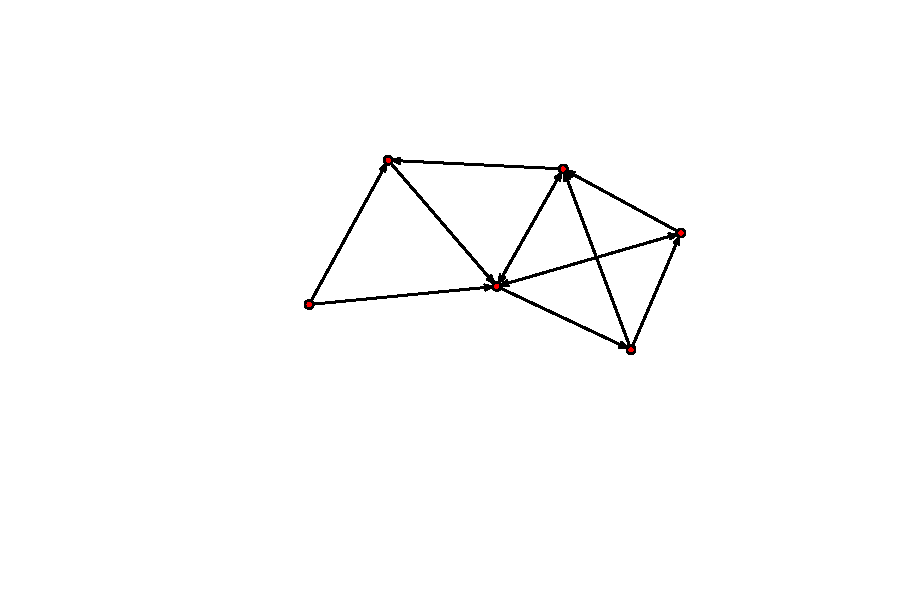
\includegraphics{enaR-vignette-014}
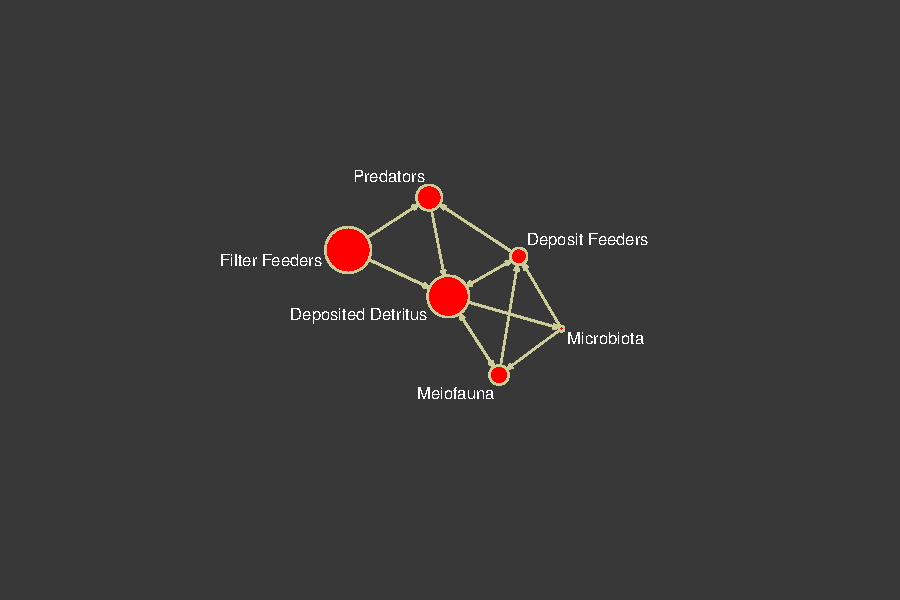
\includegraphics{enaR-vignette-015}
\caption{Two networks for the Oyster Reef model
  \citep{dame81} showing a simple (left) and more elaborate (right)
  implementation of the network plotting function.} \label{fig:oyster}
\end{figure}




%%3. model input

\subsection{Data Input: Reading Common Data File Formats}
Several software packages exist in the literature for running ENA.  For
convenience, we have written functions to read in a few of the more
common data formats used by these software.

\subsection*{SCOR}
The \texttt{read.scor} function reads in data stored in the SCOR
format specified by \citet{ulanowicz91} that is the input to the
NETWRK4 programs.  This function can be run as follows.

\begin{Schunk}
\begin{Sinput}
> scor.model <- readLines('http://people.uncw.edu/borretts/data/oyster.dat')
> m <- read.scor(scor.model,from.file=FALSE)
\end{Sinput}
\end{Schunk}

This constructs the network data object from the SCOR file that stores
the ecosystem model data for an oyster reef model \citep{dame81}.  The
individual model elements are

\begin{Schunk}
\begin{Sinput}
> unpack(m)
\end{Sinput}
\begin{Soutput}
$F
                   Filter Feeders Microbiota Meiofauna Deposit Feeders
Filter Feeders                  0     0.0000    0.0000          0.0000
Microbiota                      0     0.0000    1.2060          1.2060
Meiofauna                       0     0.0000    0.0000          0.6609
Deposit Feeders                 0     0.0000    0.0000          0.0000
Predators                       0     0.0000    0.0000          0.0000
Deposited Detritus              0     8.1721    7.2745          0.6431
                   Predators Deposited Detritus
Filter Feeders        0.5135            15.7910
Microbiota            0.0000             0.0000
Meiofauna             0.0000             4.2403
Deposit Feeders       0.1721             1.9076
Predators             0.0000             0.3262
Deposited Detritus    0.0000             0.0000

$z
[1] 41.47  0.00  0.00  0.00  0.00  0.00

$r
[1] 25.1650  5.7600  3.5794  0.4303  0.3594  6.1759

$e
[1] 0 0 0 0 0 0

$y
[1] 25.1650  5.7600  3.5794  0.4303  0.3594  6.1759

$X
[1] 2000.0000    2.4121   24.1210   16.2740   69.2370 1000.0000

$Living
[1]  TRUE  TRUE  TRUE  TRUE  TRUE FALSE
\end{Soutput}
\end{Schunk}

This same data is stored as a network data object that is distributed
with this package, which can be accessed as:
\begin{Schunk}
\begin{Sinput}
> data(oyster)
> m <- oyster
\end{Sinput}
\end{Schunk}

\subsection*{WAND}
In part to make ENA more accessible to biologists,
\citet{allesina04_wand} recoded some of Ulanowicz's NETWRK4 algorithms
into a Microsoft Excel based tool called WAND.  For this tool, the
model data is stored as a separate Excel file with two worksheets.
The first contains many of the node attributes and the second contains the
flow matrix.  The \texttt{read.wand} function will create an \R\
network data object from a WAND model file. An example WAND file can
be found at \url{http://people.uncw.edu/borretts/data/MDmar02_WAND.xls}.

\begin{Schunk}
\begin{Sinput}
> m <- read.wand('data/MDmar02_WAND.xls')